\subsection{Subpaso 1-A: Iniciar estadísticas por mes}
	En la configuración de las estadísticas se tiene que seleccionar el 
	inciso \textbf{Por mes} y el año que desea la estadística. 
		
	\begin{figure}[hbtp]

	
\includegraphics[scale=0.5]{images/Interfaz/IUGS15_configuracionMes.PNG}
	\caption{Configuración por Mes }
	\end{figure}
	A continuación se aprieta el botón \textbf{Consultar}
	
\subsection{Subpaso 1-B: Muestra de Estadísticas}
	Se mostrará la siguiente interfaz con las siguientes estadísticas:
	\begin{figure}[hbtp]
		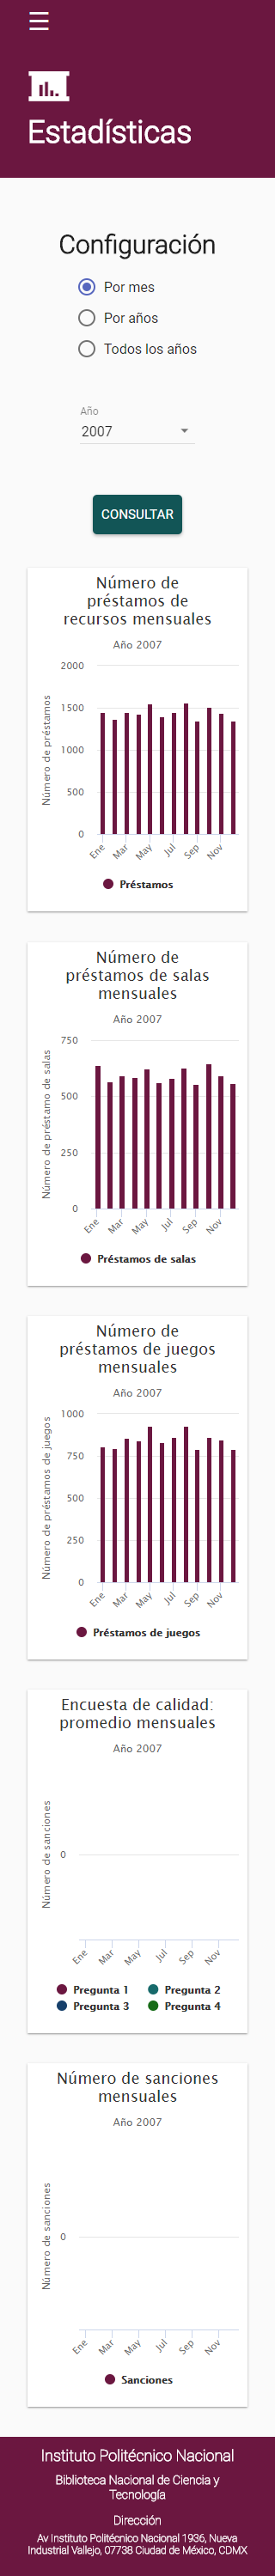
\includegraphics[scale=0.3]{images/Interfaz/IUGS15_estadisticasMes.PNG}
		\caption{Pagina general de Estadísticas por Mes}
	\end{figure}	
	
\begin{itemize}
	\item  Las estadísticas que se mostraran son las siguientes:
	\begin{enumerate}
		
		\item Número de préstamos de recursos
		\begin{figure}[hbtp]
	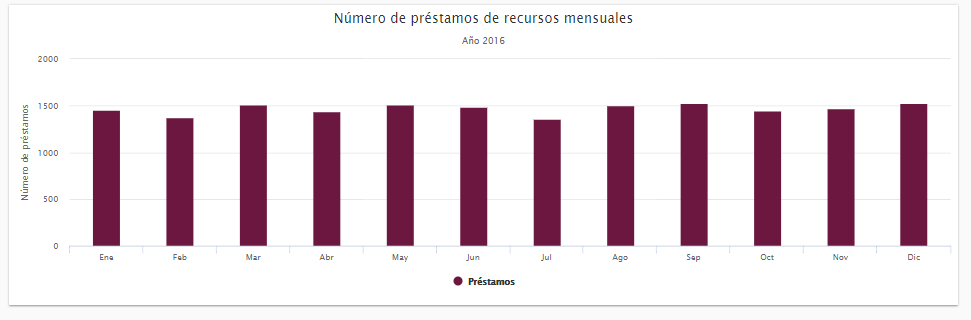
\includegraphics[scale=0.5]{images/Interfaz/IUGS15_recursosMes.PNG}
	\caption{Número de préstamos de recursos}
	\end{figure}
	
	\item Número de préstamos de salas
	\begin{figure}[hbtp]
	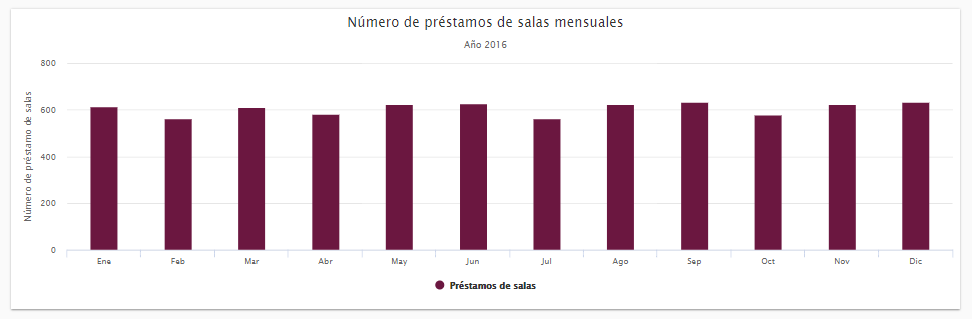
\includegraphics[scale=0.5]{images/Interfaz/IUGS15_salasMes.PNG}
	\caption{Número de préstamos de salas}
	\end{figure}
	
	\item Número de préstamos de juegos
	\begin{figure}[hbtp]
	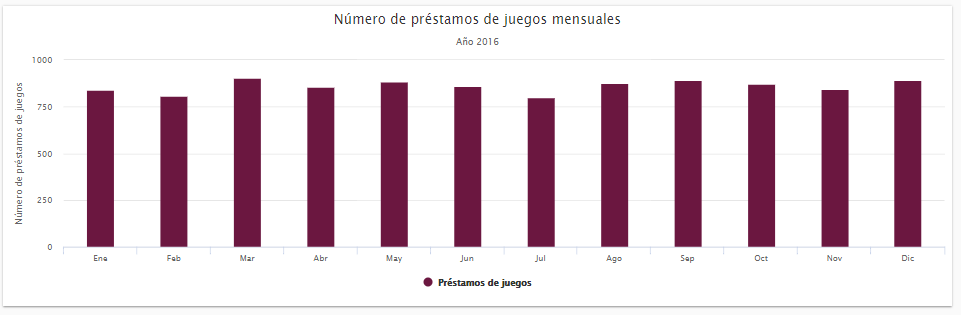
\includegraphics[scale=0.5]{images/Interfaz/IUGS15_juegosMes.PNG}
	\caption{Número de préstamos de juegos}
	\end{figure}
	
	\item Encuesta de calidad: promedio
	\begin{figure}[hbtp]
	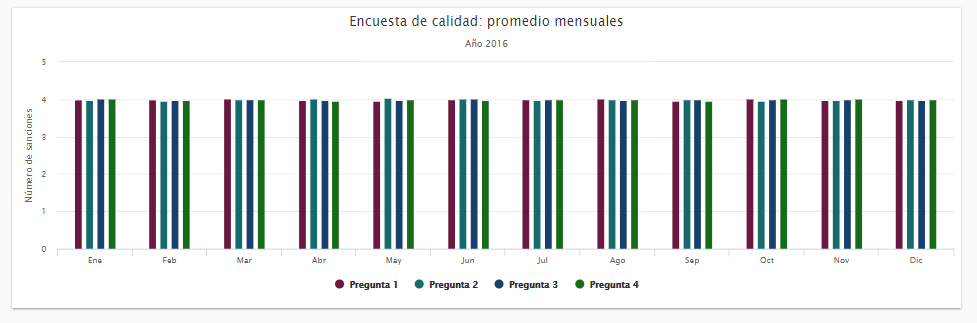
\includegraphics[scale=0.5]{images/Interfaz/IUGS15_encuestaCalidadMes.PNG}
	\caption{Encuesta de calidad: promedio}
	\end{figure}
	
	\item Número de sanciones 
	\begin{figure}[hbtp]
	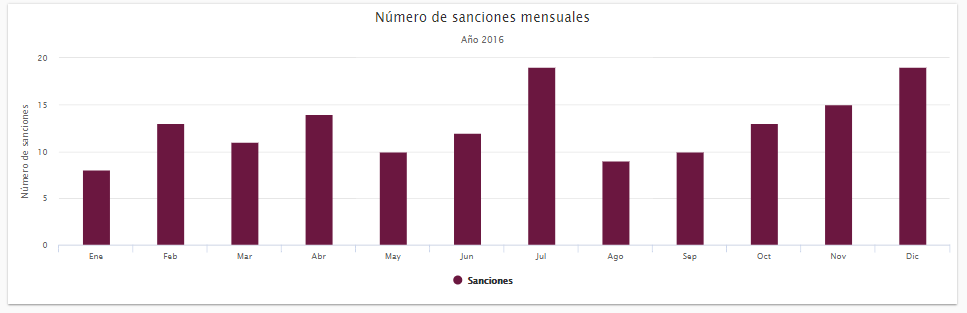
\includegraphics[scale=0.5]{images/Interfaz/IUGS15_sancionesMes.PNG}
	\caption{Número de sanciones}
	\end{figure}
	
	\end{enumerate}
	
\end{itemize}